%% BioMed_Central_Tex_Template_v1.05
%%                                      %
%  bmc_article.tex            ver: 1.05 %
%                                       %


%%%%%%%%%%%%%%%%%%%%%%%%%%%%%%%%%%%%%%%%%
%%                                     %%
%%  LaTeX template for BioMed Central  %%
%%     journal article submissions     %%
%%                                     %%
%%         <27 January 2006>           %%
%%                                     %%
%%                                     %%
%% Uses:                               %%
%% cite.sty, url.sty, bmc_article.cls  %%
%% ifthen.sty. multicol.sty		       %%
%%									   %%
%%                                     %%
%%%%%%%%%%%%%%%%%%%%%%%%%%%%%%%%%%%%%%%%%


%%%%%%%%%%%%%%%%%%%%%%%%%%%%%%%%%%%%%%%%%%%%%%%%%%%%%%%%%%%%%%%%%%%%%
%%                                                                 %%	
%% For instructions on how to fill out this Tex template           %%
%% document please refer to Readme.pdf and the instructions for    %%
%% authors page on the biomed central website                      %%
%% http://www.biomedcentral.com/info/authors/                      %%
%%                                                                 %%
%% Please do not use \input{...} to include other tex files.       %%
%% Submit your LaTeX manuscript as one .tex document.              %%
%%                                                                 %%
%% All additional figures and files should be attached             %%
%% separately and not embedded in the \TeX\ document itself.       %%
%%                                                                 %%
%% BioMed Central currently use the MikTex distribution of         %%
%% TeX for Windows) of TeX and LaTeX.  This is available from      %%
%% http://www.miktex.org                                           %%
%%                                                                 %%
%%%%%%%%%%%%%%%%%%%%%%%%%%%%%%%%%%%%%%%%%%%%%%%%%%%%%%%%%%%%%%%%%%%%%


\NeedsTeXFormat{LaTeX2e}[1995/12/01]
\documentclass[10pt]{bmc_article}    



% Load packages
\usepackage{cite} % Make references as [1-4], not [1,2,3,4]
\usepackage{url}  % Formatting web addresses  
\usepackage{ifthen}  % Conditional 
\usepackage{multicol}   %Columns
\usepackage[utf8]{inputenc} %unicode support
%\usepackage[applemac]{inputenc} %applemac support if unicode package fails
%\usepackage[latin1]{inputenc} %UNIX support if unicode package fails
\urlstyle{rm}
\usepackage{graphicx}
\usepackage{color}

 
 
%%%%%%%%%%%%%%%%%%%%%%%%%%%%%%%%%%%%%%%%%%%%%%%%%	
%%                                             %%
%%  If you wish to display your graphics for   %%
%%  your own use using includegraphic or       %%
%%  includegraphics, then comment out the      %%
%%  following two lines of code.               %%   
%%  NB: These line *must* be included when     %%
%%  submitting to BMC.                         %% 
%%  All figure files must be submitted as      %%
%%  separate graphics through the BMC          %%
%%  submission process, not included in the    %% 
%%  submitted article.                         %% 
%%                                             %%
%%%%%%%%%%%%%%%%%%%%%%%%%%%%%%%%%%%%%%%%%%%%%%%%%                     


%\def\includegraphic{}
%\def\includegraphics{}



\setlength{\topmargin}{0.0cm}
\setlength{\textheight}{21.5cm}
\setlength{\oddsidemargin}{0cm} 
\setlength{\textwidth}{16.5cm}
\setlength{\columnsep}{0.6cm}

\newboolean{publ}

%%%%%%%%%%%%%%%%%%%%%%%%%%%%%%%%%%%%%%%%%%%%%%%%%%
%%                                              %%
%% You may change the following style settings  %%
%% Should you wish to format your article       %%
%% in a publication style for printing out and  %%
%% sharing with colleagues, but ensure that     %%
%% before submitting to BMC that the style is   %%
%% returned to the Review style setting.        %%
%%                                              %%
%%%%%%%%%%%%%%%%%%%%%%%%%%%%%%%%%%%%%%%%%%%%%%%%%%
 

%Review style settings
\newenvironment{bmcformat}{\begin{raggedright}\baselineskip20pt\sloppy\setboolean{publ}{false}}{\end{raggedright}\baselineskip20pt\sloppy}

%Publication style settings
%\newenvironment{bmcformat}{\fussy\setboolean{publ}{true}}{\fussy}



% Begin ...
\begin{document}
\begin{bmcformat}


%%%%%%%%%%%%%%%%%%%%%%%%%%%%%%%%%%%%%%%%%%%%%%
%%                                          %%
%% Enter the title of your article here     %%
%%                                          %%
%%%%%%%%%%%%%%%%%%%%%%%%%%%%%%%%%%%%%%%%%%%%%%

\title{Towards speed up of Whole Genome Alignment using Distributed Suffix Tree}
 
%%%%%%%%%%%%%%%%%%%%%%%%%%%%%%%%%%%%%%%%%%%%%%
%%                                          %%
%% Enter the authors here                   %%
%%                                          %%
%% Ensure \and is entered between all but   %%
%% the last two authors. This will be       %%
%% replaced by a comma in the final article %%
%%                                          %%
%% Ensure there are no trailing spaces at   %% 
%% the ends of the lines                    %%     	
%%                                          %%
%%%%%%%%%%%%%%%%%%%%%%%%%%%%%%%%%%%%%%%%%%%%%%


\author{Julio Cesar Garcia Vizcaino\correspondingauthor$^{1}$%
       \email{Julio Cesar Garcia Vizcaino\correspondingauthor - juliocesar.garcia@e-campus.uab.cat}%
      \and
       and 
         Antonio Espinosa$^2$%
         \email{Antonio Espinosa - antonio.espinosa@caos.uab.es}%
      }
      

%%%%%%%%%%%%%%%%%%%%%%%%%%%%%%%%%%%%%%%%%%%%%%
%%                                          %%
%% Enter the authors' addresses here        %%
%%                                          %%
%%%%%%%%%%%%%%%%%%%%%%%%%%%%%%%%%%%%%%%%%%%%%%

\address{%
    \iid(1)Computer Architecture \& Operating Systems Department (CAOS), Universitat Autònoma de Barcelona,%
    Bellaterra (Barcelona), Spain.\\
    \iid(2)Computer Architecture \& Operating Systems Department (CAOS), Universitat Autònoma de Barcelona,%
    Bellaterra (Barcelona), Spain.
}%

\maketitle

%%%%%%%%%%%%%%%%%%%%%%%%%%%%%%%%%%%%%%%%%%%%%%
%%                                          %%
%% The Abstract begins here                 %%
%%                                          %%
%% The Section headings here are those for  %%
%% a Research article submitted to a        %%
%% BMC-Series journal.                      %%  
%%                                          %%
%% If your article is not of this type,     %%
%% then refer to the Instructions for       %%
%% authors on http://www.biomedcentral.com  %%
%% and change the section headings          %%
%% accordingly.                             %%   
%%                                          %%
%%%%%%%%%%%%%%%%%%%%%%%%%%%%%%%%%%%%%%%%%%%%%%


\begin{abstract}
        % Do not use inserted blank lines (ie \\) until main body of text.
        \paragraph*{Background:} Text for this section of the abstract. 
      
        \paragraph*{Results:} Text for this section of the abstract \ldots

        \paragraph*{Conclusions:} Text for this section of the abstract \ldots
\end{abstract}



\ifthenelse{\boolean{publ}}{\begin{multicols}{2}}{}




%%%%%%%%%%%%%%%%%%%%%%%%%%%%%%%%%%%%%%%%%%%%%%
%%                                          %%
%% The Main Body begins here                %%
%%                                          %%
%% The Section headings here are those for  %%
%% a Research article submitted to a        %%
%% BMC-Series journal.                      %%  
%%                                          %%
%% If your article is not of this type,     %%
%% then refer to the instructions for       %%
%% authors on:                              %%
%% http://www.biomedcentral.com/info/authors%%
%% and change the section headings          %%
%% accordingly.                             %% 
%%                                          %%
%% See the Results and Discussion section   %%
%% for details on how to create sub-sections%%
%%                                          %%
%% use \cite{...} to cite references        %%
%%  \cite{koon} and                         %%
%%  \cite{oreg,khar,zvai,xjon,schn,pond}    %%
%%  \nocite{smith,marg,hunn,advi,koha,mouse}%%
%%                                          %%
%%%%%%%%%%%%%%%%%%%%%%%%%%%%%%%%%%%%%%%%%%%%%%




%%%%%%%%%%%%%%%%
%% Background %%
%%
\section*{Background}
Today, we know that species are described by DNA, a complex molecule comprised of many smaller molecules called nucleotides. The data describing a single specie,commonly called a genome, can be millions or billions of nucleotides long.\\
One of the most basic computational tasks that we perform on genomic data is identifying the evolutionary relationships between DNA from two or more species. On a smaller scale, we wish to identify which individual nucleotides are unique to species, and which nucleotides share ancestry. On a larger scale, we look to \textbf{find entire subsequences that are a common between them}.\\
Currently the availability of a huge amount of  Bioinformatics data (often in the public domain), and on the other hand the  need for new and efficient methods and algorithms capable of  compute the information contained in the data requires the use of HPC to manipulate it. As a matter of fact, the  emphasis of research in Bioinformatics and HPC is shifting from the development of efficient data storing and handling methods, to the one of methods able to  extract useful information from data.\\
Consequently, the computational demands needed to explore and analyze the data contained in the genome databases is quickly becoming a great concern. To meet these demands, we must use high performance computing, such as parallel computers and distributed networks of workstations.\\
This paper focuses in the whole genome alignment problem. A whole genome alignment is the process of identifying a mapping from each position in query genome to its corresponding position in the reference genome.\\ 
We now describe some notation, give a more detailed introduction to whole genome alignment, and describe the mathematical framework on which we base most of techniques used to perform whole genome alignment. First we define some basic notation. We use R (Reference) and Q (Query) to denote sequences. For sequence R, we refer to position $i$ as $R_{i}$ and let the first position be $R_{0}$.\\
Sequence alignment is the primary tool for finding evolutionary relationships between DNA sequences. A DNA sequence is a string over four symbols: A, T , C, and G. These symbols represent the nucleotides adenine, thymine, cytosine, and guanine, respectively. As time passes, DNA sequences incur mutations from a variety of physical processes. Thus, DNA sequences from individuals of a specie contain many differences. When aligning DNA sequences from different species, large scale changes, such as long insertions and deletions, duplications, reversals and translocations, are common, see Figure \ref{schema}. The goal of sequence alignment is to infer which changes occurred with a mathematical model that abstracts the physical mutation processes.\\
\begin{figure}[hbp] 
  \begin{center}
      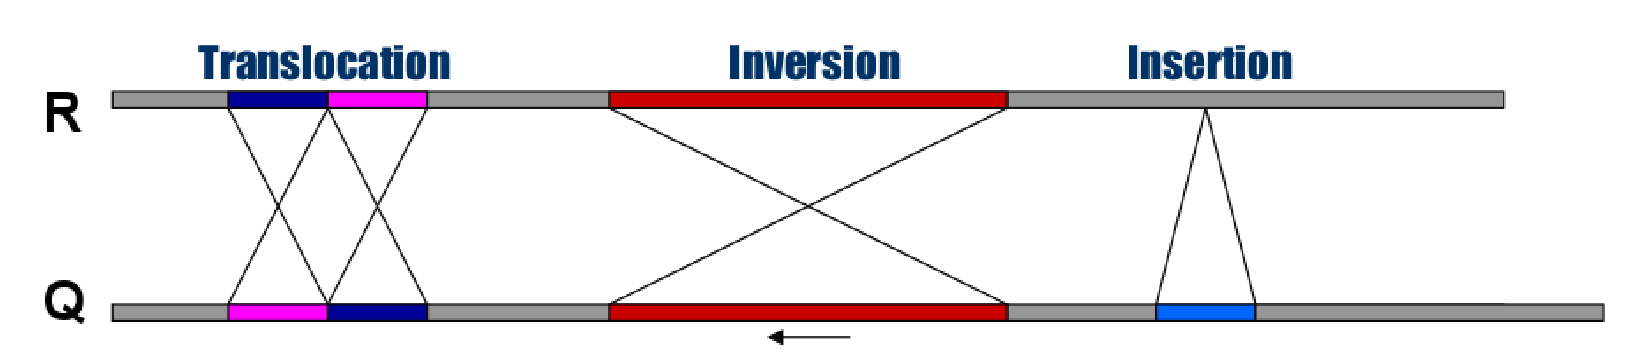
\includegraphics[scale=0.5]{schema.eps}
    \caption{Operations in whole genome alignment}
    \label{schema}
  \end{center}
\end{figure}
Given two sequences, we can interpret an alignment. We stack the aligned sequences on top of one another and look at the content of the every position, we can see the following schema:
\begin{center}
\begin{tabular}{l l}
Original sequence:& AGGCCTC \\
Mutations:& \textcolor{blue}{AGG}\textcolor{red}{A}\textcolor{blue}{CTC} \\
Insertions:& \textcolor{blue}{AGG}\textcolor{red}{G}\textcolor{blue}{CCTC} \\
Deletions:& \textcolor{blue}{AGG}\textcolor{green}{.}\textcolor{blue}{CTC} \\
\end{tabular}
\end{center}
Finding all these changes is a time-intensive operation in whole genome alignment. Moreover, the size of the genome can be an issue when there is not enough memory to store the reference and query genome.\\
The standard algorithms for sequence alignment rely on either dynamic programming or hashing techniques. Naïve versions of dynamic programming use $O(n^2)$ space and time (where n is the length of the shorter of the two sequences being compared), which makes computation simply unfeasible for sequences of size $\ge 4$ Mb. Hashing techniques operate faster on average, but they involve a ‘match and extend’ strategy, where the ‘extend’ part also takes $O(n^2)$ time. For dynamic programming, it is possible to reduce the required space to $O(n)$ by taking more time; this solves the memory problem but still leaves one with an unacceptably slow algorithm. Faster algorithms can be developed for specialized purposes.\\
More complex dynamic programming methods can be used for alignment when the alignment error is expected to be low. For example, one can align two similar sequences with at most E differences (or errors) in time proportional to E times the length of the longer sequence.
\subsection{MUMmer}
MUMmer, a widely-used bioinformatic application, is the tool that we use to solve the whole genome alignment problem. MUMmer assumes the sequences are closely related, and using this assumption can quickly compare sequences that are millions of nucleotides in length. The basis of the algorithm is a data structure known as a suffix tree, which allows one to find, extremely efficiently, all distinct subsequences in a given sequence. However the requirements of space needed to store the suffix tree in main memory make a non-viable structure when the suffix tree to be stored exceeds the available memory. The space complexity of the suffix tree used in MUMmer is $O(17n)$, where n is the length of the reference genome.\\

%%%%%%%%%%%%%%%%%%%%%%%%%%%%
%% Results and Discussion %%
%%
\section*{Results and Discussion}
  \subsection*{Results sub-heading}
    \subsubsection*{This is a sub-sub-heading}
      Sub-sub-sub-headings are made with the \textsl{\\subsubsection} command. \pb
      pb at end of lines ensures correct paragraph spacing.\pb
	  Text for this sub-sub-section \ldots
    \subsubsection*{Another sub-sub-sub-heading}
      Text for this sub-sub-section \ldots

  \subsection*{Another results sub-heading}
    Text for this sub-section \ldots

  \subsection*{Yet another results sub-heading}
    Text for this sub-section.  More results \ldots


    

%%%%%%%%%%%%%%%%%%%%%%
\section*{Conclusions}
  Text for this section \ldots


  
%%%%%%%%%%%%%%%%%%
\section*{Methods}
  \subsection*{Methods sub-heading for this section}
    Text for this sub-section \ldots

  \subsection*{Another methods sub-heading for this section}
    Text for this sub-section \ldots

  \subsection*{Yet another sub-heading for this section}
    Text for this sub-section \ldots


    
%%%%%%%%%%%%%%%%%%%%%%%%%%%%%%%%
\section*{Authors contributions}
    Text for this section \ldots

    

%%%%%%%%%%%%%%%%%%%%%%%%%%%
\section*{Acknowledgements}
  \ifthenelse{\boolean{publ}}{\small}{}
  Text for this section \ldots


 
%%%%%%%%%%%%%%%%%%%%%%%%%%%%%%%%%%%%%%%%%%%%%%%%%%%%%%%%%%%%%
%%                  The Bibliography                       %%
%%                                                         %%              
%%  Bmc_article.bst  will be used to                       %%
%%  create a .BBL file for submission, which includes      %%
%%  XML structured for BMC.                                %%
%%                                                         %%
%%                                                         %%
%%  Note that the displayed Bibliography will not          %% 
%%  necessarily be rendered by Latex exactly as specified  %%
%%  in the online Instructions for Authors.                %% 
%%                                                         %%
%%%%%%%%%%%%%%%%%%%%%%%%%%%%%%%%%%%%%%%%%%%%%%%%%%%%%%%%%%%%%


{\ifthenelse{\boolean{publ}}{\footnotesize}{\small}
 \bibliographystyle{bmc_article}  % Style BST file
  \bibliography{bmc_article} }     % Bibliography file (usually '*.bib' ) 

%%%%%%%%%%%

\ifthenelse{\boolean{publ}}{\end{multicols}}{}

%%%%%%%%%%%%%%%%%%%%%%%%%%%%%%%%%%%
%%                               %%
%% Figures                       %%
%%                               %%
%% NB: this is for captions and  %%
%% Titles. All graphics must be  %%
%% submitted separately and NOT  %%
%% included in the Tex document  %%
%%                               %%
%%%%%%%%%%%%%%%%%%%%%%%%%%%%%%%%%%%

%%
%% Do not use \listoffigures as most will included as separate files

\section*{Figures}
  \subsection*{Figure 1 - Sample figure title}
      A short description of the figure content
      should go here.

  \subsection*{Figure 2 - Sample figure title}
      Figure legend text.



%%%%%%%%%%%%%%%%%%%%%%%%%%%%%%%%%%%
%%                               %%
%% Tables                        %%
%%                               %%
%%%%%%%%%%%%%%%%%%%%%%%%%%%%%%%%%%%

%% Use of \listoftables is discouraged.
%%
\section*{Tables}
  \subsection*{Table 1 - Sample table title}
    Here is an example of a \emph{small} table in \LaTeX\ using  
    \verb|\tabular{...}|. This is where the description of the table 
    should go. \par \mbox{}
    \par
    \mbox{
      \begin{tabular}{|c|c|c|}
        \hline \multicolumn{3}{|c|}{My Table}\\ \hline
        A1 & B2  & C3 \\ \hline
        A2 & ... & .. \\ \hline
        A3 & ..  & .  \\ \hline
      \end{tabular}
      }
  \subsection*{Table 2 - Sample table title}
    Large tables are attached as separate files but should
    still be described here.



%%%%%%%%%%%%%%%%%%%%%%%%%%%%%%%%%%%
%%                               %%
%% Additional Files              %%
%%                               %%
%%%%%%%%%%%%%%%%%%%%%%%%%%%%%%%%%%%

\section*{Additional Files}
  \subsection*{Additional file 1 --- Sample additional file title}
    Additional file descriptions text (including details of how to
    view the file, if it is in a non-standard format or the file extension).  This might
    refer to a multi-page table or a figure.

  \subsection*{Additional file 2 --- Sample additional file title}
    Additional file descriptions text.


\end{bmcformat}
\end{document}







